\documentclass{article}       % use "amsart" instead of "article" for AMSLaTeX format
\usepackage{geometry}                              % See geometry.pdf to learn the layout options. There are lots.
%\geo4metry{landscape}                            % Activate for for rotated page geometry
%\usepackage[parfill]{parskip}                  % Activate to begin paragraphs with an empty line rather than an indent
\usepackage{graphicx}                         % Use pdf, png, jpg, or eps§ with pdflatex; use eps in DVI mode
% TeX will automatically convert eps --> pdf in pdflatex         
\usepackage{amssymb}
\usepackage{amsmath}
\usepackage{mathtools}
\usepackage{booktabs}
\usepackage{tabto}
\usepackage{algorithm}
%\usepackage{algorithmic}
\usepackage{algpseudocode}
\usepackage{tikz}

\usetikzlibrary{shapes.geometric}



\title{Adv Data Struct $\&$ Algorithm: Homework 2}
\author{Zimian Li}

\begin{document}
        
\maketitle

\begin{enumerate}
	\item[1.] A GRE combined score is an iteger between 260 and 340. You are given a sorted array with the scores of all the n students that took the exam in 2017. Design and analyze a sublinear (i.e., in o(n)) algorithm that reports the number of people that received each score x, for $260 \leq x \leq 340$.\newline\newline
	The algorithm is as below. FindUpper is like binary search, thus apparently the time complexity of function FindUpper is $\Theta (log(n))$. The function CountScores executes 80 times of FindUpper, so its time complexity is also  $\Theta (log(n))$.\newline
	I also compared it with a naive brute force algorithm with $\Theta (n)$ time cost. I just counted the times of loops in these 2 algorithms. As it shows below, when n is small, the brute force algorithm has a smaller number of loops and runs faster. That is because CountScores has a big constant factor. When n is big enough, it's easy to find the time cost of my algorithm grows much slower than the brute force one.\newline
	\begin{figure}[H]
		\centering
		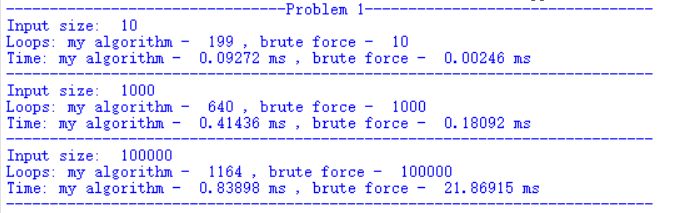
\includegraphics[width=15cm]{p1}
		\caption{(p1)}
		\label{p1}
	\end{figure}
	 \begin{algorithm}[H]
		\caption{Count Scores}
		\small
		\begin{algorithmic}[1]
			\Procedure {FindUpper}{A, x, p, r}
			\State mid = (p+r)/2
			\If {p == r}
			\If {A[mid] == x}
			\State return mid
			\Else \State \Return None
			\EndIf
			\Else \If {A[mid] == x and A[mid+1] $>$ A[mid]}
			\State \Return mid
			\EndIf
			\If {A[mid] $>$ x}
			\State \Return FindUpper(A, x, p, mid-1)
			\EndIf
			\If {(A[mid] $<$ x) or ((A[mid] == x) and (A[mid+1] == x)}
			\State \Return FindUpper(A, x, mid+1, r)
			\EndIf
			\EndIf
			\EndProcedure
			
			\Procedure {CountScores}{A}
			\State initialize a hashmap Result
			\State lower = 0, upper = 0
			\For {x $\gets$260 to 340}
			\State 	upper = FindUpper(A, x, lower, len(A)-1)
			\If {upper == None}
			\State Result[x] = 0
			\Else
			\State Result[x] = upper - lower + 1
			\State lower = upper + 1
			\EndIf
			\EndFor
			\State \Return Result
			\EndProcedure
		\end{algorithmic}\label{p1}
	\end{algorithm}
	\item[2.] Let S be a set of n points in ${\mathbb{R}}^2$. The bounding box of S is the smallest upright rectangle containing S.\newline
	\begin{enumerate}
		\item[(a)] Describe and analyze a divide-and-conquer algorithm to compute the bounding box of n points in the plane using fewer than 3n element to element comparisons. Make sure that your solution handles correctly all values of n.\newline
		\begin{algorithm}[H]
			\caption{Find the bounding box}
			\small
			\begin{algorithmic}[1]
				\Procedure {FindBoundingBox}{A, p, r}
				\State minX, maxX, minY, maxY = 0
				\If {r - p == 1}
				\If {A[p][0] $<$ A[r][0]}
				\State minX = A[p][0]
				\State maxX = A[r][0]
				\Else
				\State minX = A[r][0]
				\State maxX = A[p][0]
				\EndIf
				\If {A[p][1] $<$ A[r][1]}
				\State minY = A[p][1]
				\State maxY = A[r][1]
				\Else
				\State minY = A[r][1]
				\State maxY = A[p][1]
				\EndIf
				\State \Return minX, maxX, minY, maxY
				\EndIf
				\If {p == r}
				\State \Return A[p][0], A[p][1], A[p][0], A[p][1]
				\EndIf
				\State mid = (p+r)/2
				\If {mid is even}
				\State mid += 1
				\EndIf
				\State minX, maxX, minY, maxY = FindBoundingBox(A, p, mid)
				\State  minX1, maxX1, minY1, maxY1 = FindBoundingBox(A, mid+1, r)
				\State minX = min(minX, minX1)
				\State minY = min(minY, minY1)
				\State maxX = max(maxX, maxX1)
				\State maxY = max(maxY, maxY1)
				\State \Return minX, maxX, minY, maxY
				\EndProcedure
			\end{algorithmic}\label{p2}
		\end{algorithm}
		Actually, for an array with $n$ points $\{(x_0, y_0), (x_1, y_1), ..., (x_n, y_n)\}$, finding an upright bounding box is equal to find the minimal and maximal values of $x$ and $y$.\newline
		The number of comparisons of my algorithm depends on the parity of $n$. If $n$ is even, then the number of comparisons is $3n - 4$, and if $n$ is odd, it's $3n - 3$, both fewer than $3n$.\newline
		I also compared it with a naive brute force algorithm as below. The brute force one takes around $4n$ times of comparisons.\newline
		\begin{figure}[H]
			\centering
			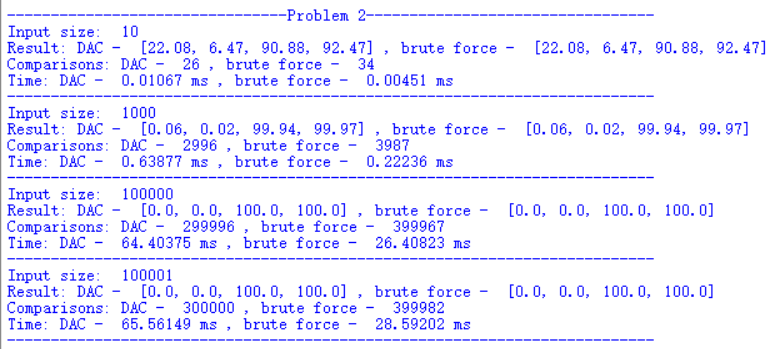
\includegraphics[width=15cm]{p2}
			\caption{(p2)}
			\label{p2}
		\end{figure}
		\item[(b)] Can an incremental approach based on adding one point at a time improve or match the performance? How about adding several points at a time? Explain.\newline\newline
		No, it can't. If we add one point at a time, this point would have to compare with current min and max values of x and y, so at last it need less than $4n$ times of comparisons. (But on the other hand in best case it only need $2n$ times of comparisons.)\newline
		But if adding several points at a time, it can match the performance, actually, if adding 2 points at a time, it could be same as the DAC algorithm, these 2 points compares first, then separately compares with min and max values of x and y. And 2 points one time is the best case, if adding more than 2 points at a time, we can't get a fewer times of comparisons.\newline 
	\end{enumerate}
	\item[3.] You are given a list A of n computational tasks that can be executed in parallel. Each task is specified by the amount of time (an integer) required to execute the task. Your goal is to assign a list of consecutive tasks to each of $p \leq n$ processors so as to minimize the total parallel processing time, i.e., the max over all p processors of the time required by each processor to solve its assigned tasks. For example, if A = $\{7, 4, 3, 5\}$ and p = 3 an optimal partition is $\{(7), (4, 3), (5)\}$ with a total parallel time of 7.
	\begin{algorithm}[H]
		\caption{Find the optimal partition}
		\small
		\begin{algorithmic}[1]
			\Procedure {minProc}{A, t}
			\State initialize a list Procs
			\State cap = 0
			\For {i $\gets$ 0 to len(A)}
			\State cap += A[i]
			\If {i == len(A) - 1}
			\State Procs.append(i)
			\Else
			\If {cap + A[i+1] $>$ t}
			\State cap = 0
			\State Procs.append(i)
			\EndIf
			\EndIf
			\EndFor
			\State \Return Procs
			\EndProcedure
			\Procedure {minTime} {A, p}
			\State approx = max(ceil(sum(A)/p), the max value in A)
			\State procs = minProc(A, approx)
			\While {len(procs) $>$ p}
			\State approx += 1
			\State procs = minProc(A, approx)
			\EndWhile
			\State \Return procs
			\EndProcedure
		\end{algorithmic}\label{p3}
	\end{algorithm}
	The first part of this algorithm is that given t to get a minimal p. It's a greedy algorithm, and the time complexity is $\Theta (n)$. However, the goal is to get a minimal t with a given p. So we need to find a lower bound of t and then iterate the first function many times until meeting the right p.\newline
	The time complexity of the whole algorithm is not easy to get. I can find a lower bound that is max(ceil(sum(A)/p), the max value in A). What about upper bound? It's easy to find $T(minTime(A, p)) \leq  T(minTime(A, p-1)) \leq ... \leq T(minTime(A, 1)) = sum(A)$. Hence, $T(minTime(A, p)) \leq (sum(A)-sum(A)/p)\cdot \Theta (n) \in O((p-1)/p \cdot sum(A) \cdot n)$. Other than $n$ and $p$, it's related with the content of the input array.
	\begin{figure}[H]
		\centering
		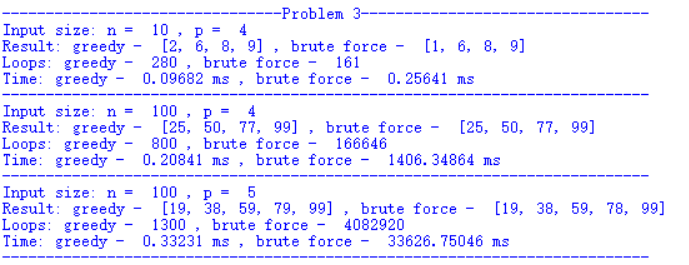
\includegraphics[width=15cm]{p3}
		\caption{(p3)}
		\label{p3}
	\end{figure}
	Compared with a brute force algorithm of which time complexity is $O({{n-1}\choose{p-1}} \cdot n)$, when the input size gets bigger, it has a much better performance than the brute force one.\newline
	 
	\item[4.] The problem of finding local maxima of a function $f : \mathbb{R} \to \mathbb{R}$ finds numerous applications in fields as varied as machine learning and anthropology. We are interested here in the discrete version of this problem, where $f$ is represented as an array of number, A location in A is a local maximum if its value is greater than or equal to that of its immediate neighbors. As an example, given an elevation raster of a terrain, an archaeologist may be interested in locating the location of mounds, as they may correspond to a promising excavation sites.\newline
	\begin{enumerate}
		\item[(a)] In the 1D version of this problem, you are given an array A of n numbers. A[k] is a local maximum if $A[k-1] \leq A[k]$ and $A[k] \geq A[k+1]$ (adjusting accordingly, if A[x] only has one neighbor). For example, the array (9, 7, 7, 2, 1, 3, 7, 5, 4, 7, 3, 3, 4) has four local maxima (at location 1, 3, 7, and 10).
		\begin{enumerate}
			\item [i.] Prove that a local maximum must exist.\newline
			\textbf{Proof:} Assume there's no local maximum in the array A. Then for any element in the array A except head and tail, it has to meet $A[k-1] < A[k] < A[k+1], or A[k-1] > A[k] > A[k+1], or A[k] < A[k-1] and A[k] < A[k+1]$. And for the head element $A[0]$, it has to meet $A[0] < A[1]$, then for $A[1]$, it has already greater than $A[0]$, so we can conclude $A[1] < A[2]$, the consider $A[2]$, and repeat this process to the end, then we can find for the tail $A[n-1]$, $A[n-1] > A[n-2]$, so $A[n-1]$ is a local maxima, that's a contradiction! Hence, a local maximum must exist.\newline
			\item[ii.] Describe and analyze an agorithm that finds a local maximum in $o(n)$ time.
			\begin{algorithm}[H]
				\caption{Find a local maximum in 1D array}
				\small
				\begin{algorithmic}[1]
					\Procedure {findLocalMax1D}{A, p, r}
					\State mid = (p+r)/2
					\If {mid == 0 and A[mid] $\geq$ A[mid+1]}
					\State \Return mid
					\Else \If {mid == len(A)-1 and A[mid] $\geq$ A[mid-1]}
					\State \Return mid
					\EndIf
					\If {A[mid] $\geq$ A[mid-1] and A[mid] $\geq$ A[mid+1]}
					\State \Return mid
					\EndIf
					\If {A[mid] $< $A[mid-1]}
					\State \Return findLocalMax1D(A, p, mid-1)
					\EndIf
					\State \Return findLocalMax1D(A, mid+1, r)
					\EndIf
					\EndProcedure
				\end{algorithmic}\label{p4}
			\end{algorithm}
		It's similar with binary search, takes $\Theta (log n)$ time.
		\begin{figure}[H]
			\centering
			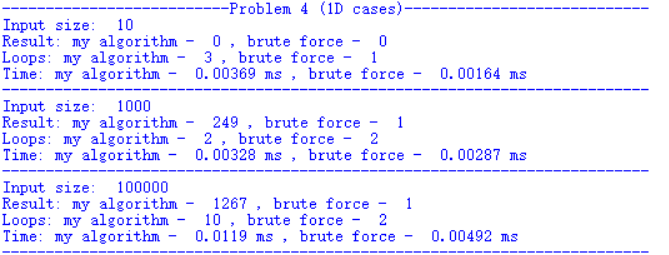
\includegraphics[width=15cm]{p41}
			\caption{(p41)}
			\label{p41}
		\end{figure}
		Compared with a naive brute force algorithm, I found the brute force algorithm is also fast, which is incredible! Actually it makes sense. Consider an array with n distinct numbers, for all position except head and tail, the possibility of that an arbitrary element is a local maximum is $1/3$, for head and tail, it's $1/2$. So if we search from the head, the expected number of search times is less than $3$! If there are same numbers, it just decreases this expected value. Hence, in average case, the brute force algorithm is a $\Theta (1)$ algorithm, it's really fast. It's the same for my binary search. But in the worst case, the brute force algorithm would take $\Theta (n^2)$, not that much good.\newline
		\end{enumerate}
		\item[(b)] In 2D, you are given a $n \times n$ array A of numbers. Then A[i, j] is a local maimum if it is greater than or equal to its four neighbors: A[i - 1, j], A[i + 1, j], A[i, j - 1], A[i, j + 1]. Describe and analyze an algorithm that finds a local maimum in $o(n^2)$ time.
		\begin{algorithm}[H]
			\caption{Find a local maximum in 2D array}
			\small
			\begin{algorithmic}[1]
				\Procedure {findLocalMax2D}{A, p, r}
				\State mid = (p+r)/2
				\State maxy = max(A[mid])
				\If {mid == 0 and A[mid][maxy] $\geq$ A[mid+1][maxy]}
				\State \Return mid, maxy
				\Else \If {mid == len(A)-1 and A[mid][maxy] $\geq$ A[mid-1][maxy]}
				\State \Return mid, maxy
				\EndIf
				\If {A[mid][maxy] $\geq$ A[mid-1][maxy] and A[mid][maxy] $\geq$ A[mid+1][maxy]}
				\State \Return mid, maxy
				\EndIf
				\If {A[mid][maxy] $< $A[mid-1][maxy]}
				\State \Return findLocalMax2D(A, p, mid-1)
				\EndIf
				\State \Return findLocalMax2D(A, mid+1, r)
				\EndIf
				\EndProcedure
			\end{algorithmic}\label{p4}
		\end{algorithm}		
	\end{enumerate}
	For this algorithm, I think I need to prove its correctness.\newline
	\textbf{Proof of Correctness:} In this algorithm, It's equal to do a binary search among the maximal values of all rows. I need to prove at least one of them is a local maximum.\newline
	Assume none of them is a local maximum. Note them as $\{A[0][k_0], A[1][k_1], ..., A[n-1][k_{n-1}]\}$. Then all of them need to meet $A[i][k_i] < A[i-1][k_i] or A[i][k_i] < A[i+1][k_i]$. Let $A[m][k_m]$ be the maximal one of all, thus I can get $A[m-1][k_m] > A[m][k_m] or A[m+1][k_m] > A[m][k_m]$. Suppose $A[m-1][k_m] > A[m][k_m]$, because $A[m-1][k_{m-1}]$ is the max of $A[m-1]$, $A[m-1][k_{m-1}] > A[m-1][k_m] \implies A[m-1][k_{m-1}] >  A[m][k_m]$. But  $A[m][k_m]$ is the maximal value of all, that's a contradiction!\newline
	So at least one of them is a local maximum, and through binary search, I can find it.\newline
	\begin{figure}[H]
		\centering
		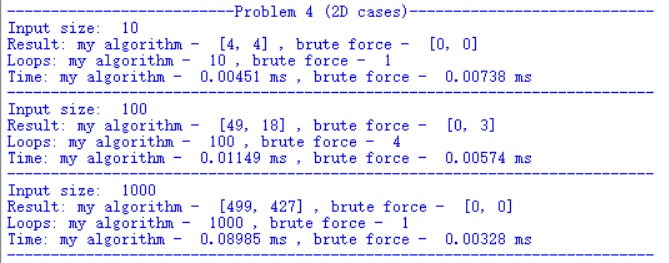
\includegraphics[width=15cm]{p42}
		\caption{(p42)}
		\label{p42}
	\end{figure}
	The time complexity of this algorithm is $\Theta(nlog(n))$. And in average case, it's worse than the brute force algorithm, for the expected value of search times of brute force algorithm is less than $5\in \Theta(1)$, but mine is $\Theta (n)$. In worst case, brute force is $\Theta (n^2)$, and mine is $\Theta (nlog(n))$. 
	\item[5.] Implement two of the algorithms (from 1, 2a, 3, 4b) in Python, Java, or C++. Compare the performance with a reasonable naive brute force algorithm, Include, in each case, a driver function that takes at least the input size n as a parameter, generates a random test case of that size, and reports the answers and running time of both your algorithm and the brute force solution. You must do this part of the assignment strictly individually.\newline\newline
	I implemented them all. Just check the attached python codes.
\end{enumerate}  
\end{document}